\chapter{}\label{Ane2}
Se presenta a continuación resultados extraídos de un modelo generado en el marco de la unidad curricular Dinámica de Estructuras. Este consiste en un análisis dinámico 2D y 3D de elementos de biela no lineales con un análisis modal complementario.  


\section{Modelado dinámico de un conductor de alta tensión utilizando elementos de barra}
\subsection{Fundamentos teóricos}

\subsubsection{Ecuación de movimiento}

En este trabajo se utilizará el principio de D’Alambert para establecer las ecuaciones de movimiento de un elemento de barra axial, este es el equivalente dinámico al Principio de los Trabajos Virtuales para el caso estático. A continuación se notará las variables posición, desplazamiento, deformación unitaria y tensión como $(x, u_t ,\epsilon_t,\sigma_t )$  y las derivadas parciales, velocidad y aceleración con $(\dot{u_t} , \ddot{u_t})$.



Dicho lo anterior el principio de D’Alambert afirma que $\forall t$ y $\forall \delta u $ se cumple:
\begin{equation}\label{dalambert}
	\int_{V_t}\sigma_t\delta \varepsilon dV_t=\int_{V_t}\delta u^Tb_{ext,t}dV_t-\int_{V_t}\rho\delta u^T\ddot{u} dV_t
\end{equation}


En la ecuación \eqref{dalambert} $b_{ext,t}$ corresponde a la fuerzas externas por unidad de volumen. El primer termino que aparece restando es el de a las fuerzas inerciales siendo $\rho$ la densidad del material. El segundo corresponde a disipaciones viscosas donde $c>0$. Esta disipación se corresponde con fenómenos de disipación estructural y rozamiento en juntas,  su valor se ajustará de acuerdo con resultados experimentales publicados, no se determinará mediante un resultado teórico. Aplicando una discretización en elementos finitos obtenemos la ecuación de movimiento de la estructura:

\begin{equation}\label{newton}
	M\ddot{u_t}+C\dot{u_t}+K_T(u_t)u_t=f_{ext,t}
\end{equation}

Las cargas externas dinámicas se encuentran asociadas con el vector $f_{ext,t}$. La matriz de rigidez $K(u_t)$ se hallará considerando no linealidad geométrica por ende tiene la siguiente forma:
\begin{equation}
	K_T=K_{T1}+K_{T2}+K_{\sigma} 
\end{equation}
\begin{equation}
	K_{T1}=EA_ol_ob_1^Tb_1
\end{equation}
\begin{equation}
	K_{T2}=EA_ol_o(b_1^Tb_2+b_2^Tb_1+b_2^Tb_2)
\end{equation}
\begin{equation}
	K_{\sigma}=\frac{\sigma A_o}{l_o}G
\end{equation}

En las ecuaciones anteriores $b_1$ y $b_2$ contienen a las derivadas de las funciones de ponderación de $u_t$  mientras que G es la matriz de Green. La matriz $K_{T1}$ es la matriz de rigidez lineal, esta no depende del desplazamiento, $K_{T2}$ es la llamada matriz de desplazamiento inicial y $K_{\sigma}$ la matriz geométrica o de tensión inicial.  

La matriz de masa M puede ser del tipo consistente o concentrada, la primera de ellas se deduce a partir de las funciones de interplación de $u_t$ $(N_i)$, mientras que la segunda se obtiene a partir de concentrar la masa de cada elemento sobre sus nodos, este último sera el utilizado para este trabajo. En el caso de una barra bidimensional tiene la siguiente forma: 
\begin{equation}
	M^e=\frac{\rho A_ol_o}{2}\begin{bmatrix}
		1&0  &0  &0 \\ 
		0& 1 &0  & 0\\ 
		0& 0 &1  &0 \\ 
		0& 0 & 0 & 1
	\end{bmatrix} 
\end{equation}


Por último la matriz C se considero de forma diagonal, para un elemento de barra:
\begin{equation}
	C^e=c \begin{bmatrix}
		1&0  &0  &0 \\ 
		0& 1 &0  & 0\\ 
		0& 0 &1  &0 \\ 
		0& 0 & 0 & 1
	\end{bmatrix} 
\end{equation}
Como se dijo anteriormente el valor de c se ajustará empíricamente de acuerdo a resultados experimentales de \cite{stengel2017measurements}.
\subsubsection{Método de diferencias centradas}
En este apartado se presenta el método por el cual se resuelve la ecuación de movimiento, se eligió este método debido a su simplicidad y su bajo coste computacional. Es de tipo explicito por ende se debe conocer la solución a la ecuación de movimiento en el tiempo $t$ para hallarse luego ${t+\Delta t}$, de acuerdo con esto último la velocidad y aceleración se escriben de la siguiente manera:
\begin{eqnarray}
	\dot{u_t}&=&\frac{u_{t+\Delta t}-u_{t-\Delta t}}{2 \Delta t}\\
	\ddot{u_t}&=&\frac{u_{t+\Delta t}+u_{t-\Delta t}-2u_t}{ \Delta t^2}
\end{eqnarray}

Sustituyendo las ecuaciones anteriores en la ecuación de movimiento y agrupando según los desplazamientos en los diferentes espacios temporales:
\begin{equation}
	\left[\frac{1}{\Delta t^2}M+\frac{1}{2\Delta t}C\right]u_{t+\Delta t}=f_{ext,t}-\left[K_T-\frac{2}{\Delta t^2}M\right]u_t-\left[\frac{1}{\Delta t^2}M-\frac{1}{2\Delta t}C\right]u_{t-\Delta t}
\end{equation}

Notar que la aproximación de la velocidad y la aceleración en el instante t induce un error de truncamiento, en segunda medida se induce un error adicional ya que $u_{t+\Delta t}$ no  verifica la ecuación dinámica de equilibrio en el instante $t+\Delta t$ sino la del instante $t$. Mencionados errores pueden ser disminuidos al reducirse el incremento temporal $\Delta t$, además condiciones de estabilidad del método para el caso lineal, donde $K_T $ no es función del desplazamiento, impone que $\Delta t<T_{min}/\pi$ donde $T_{min}$ es el mínimo periodo de vibración natural del modelo de elementos finitos.

La matriz tangente de desplazamiento y esfuerzo inicial son  función del desplazamiento, como consecuencia deben tenerse en cuenta que un incremento en la rigidez del sistema, conforme avanza el tiempo, conllevará a modos normales con mayor frecuencia y por tanto a un paso temporal crítico menor. El valor $\Delta t$ debe elegirse de acuerdo a este compromiso entre disminuir el error, permaneciendo dentro de la zona de estabilidad del método y el costo computacional.


\begin{itemize}
	\item Se presenta un algoritmo  del código utilizado:
	\begin{enumerate}
		\item Ensamblar: $M$ y $C$ a nivel de estructura.
		\item Definir tiempo final del análisis dinámico $t_f$.
		\item Definir condiciones iniciales $u_o$ y $\dot{u}_o$
		\item Calcular: $\ddot{u}_o\leftarrow M^{-1}(f_{ext,t}-C\dot{u_o}-f_{int}(u_o))$
		\item Definir  $\delta t$, considerando el compromiso mencionado anteriormente
		\item Calcular $a_o\leftarrow 1/\Delta t^2, a_1\leftarrow 1/(2\Delta t),a_2\leftarrow 2a_o,a3\leftarrow 1/a_2$
		\item Calcular $a_o\leftarrow 1/\Delta t^2, a_1\leftarrow 1/(2\Delta t),a_2\leftarrow 2a_o,a3\leftarrow 1/a_2$
		\item Calcular $u_{-\Delta t}\leftarrow u_o-\Delta \dot{u_o}_o+a_3\ddot{u_o} $
		\item Calcular y factorizar $\hat{M}=a_oM+a_1C $
		\item \textbf {while} $t<t_f$
		\item   \hspace{1cm} Calcular $\check{f_t}\leftarrow f_{ext,t}-f_{int}(u_t)+a_2Mu_t-(a_oM-a_1C)u_{t-\Delta t}$
		\item \hspace{1cm} Resolver: $ u_{t+\Delta t}\leftarrow \tilde{M}^{-1}\hat{f_t}$
		\item \hspace{1cm} Calcular la aceleración $\ddot {u_t}\leftarrow a_o(u_{t+\Delta t}-u_{t-\Delta t}-2u_t)$
		\item \hspace{1cm} Calcular la velocidad $\dot {u_t}\leftarrow a_1(u_{t+\Delta t}-u_{t-\Delta t})$
		\item\hspace{1cm} $t\leftarrow t+\Delta t$
		\item \textbf {end while}
	\end{enumerate}
\end{itemize}


\subsubsection{Modos normales}
El análisis dinámico de los modos se vuelve fundamental, este busca las soluciones a la oscilación libre no forzada, de forma que estas sean sinusoidales con determinada frecuencia natural $\omega_n$, por ende las soluciones toman la siguiente expresión $\sin (\omega_n t) \phi$. El vector $\phi$ representa un vector de escala entre las amplitudes de los desplazamientos nodales de los grados de libertad de la estructura.


La ecuación de movimiento, en complejos, de la estructura suponiendo movimientos de la forma $U(t)=\phi \exp{i\omega_n( t-t_o)}$ 
\begin{equation}\label{modos}
	\omega_n^2M\phi = K\phi
\end{equation}


La ecuación \eqref{modos} (sin amortiguamiento ni fuerzas extremas) se responde con un sistema de valores propios para una matriz simétrica y definida positiva. De forma matricial los modos normales de la estructura verifican:
\begin{equation}
	M \Phi \Omega =K\Phi
\end{equation}


Donde $\Phi $ es una matriz que tiene como columnas los vectores propios asociados a las amplitudes de los modos $\phi$ y $\Omega$ es una matriz diagonal con las frecuencias angulares de los modos $\omega_n^2$.

\subsubsection{Modelo de viento}


El flujo del viento se asume que solo tiene componente en la dirección $z$, este flujo se puede desglosar en una parte media en el tiempo y una componente fluctuante, por ende la velocidad toma la siguiente forma: $u_v(z,t)=u_m(z,t)+{u}'(z,t)  $ donde 
\begin{equation}
	u_m=\frac{1}{T}\int_{0}^{T}u_v(z,t)dt
\end{equation}


El valor del periodo $T$ debe elegirse de forma de minimizar la desviación estándar de la intensidad de turbulencia, esta se define como el cociente entre la desviación estándar de la velocidad y la velocidad media para un instante de tiempo dado.

El aire se modelará como un fluido incompresible newtoneano cuya fuerza de drag se puede escribir como:

\begin{equation}
	F_v=\int _{dl}\frac{1}{2}\rho (T)C_d(Re)d_cu_m^2(z,t)dx
\end{equation}



La fuerza de lift, en dirección perpendicular al flujo se considera despreciable frente a la fuerza de arrastre. Esta simplificación también se acompasa con la mayor rigidez del cable en la dirección perpendicular al flujo y el peso que se opone a la fuerza de sustentación. 


Existe un efecto en la dirección perpendicular al flujo  llamado "Aeolian". En dicha dirección se generan desprendimientos de vórtices asociados con la frecuencia de Strouhal $f_s=0.0925\frac{v_m}{d_c}$, cuando estos vórtices se acercan a la frecuencias naturales del cable podrían producirse resonancias, magnificándose las amplitudes del movimiento. Según \cite{Belloli2006} estos efectos deben ser considerados para velocidades medias de viento menores $6\frac{m}{s}$ , para el estudio de este trabajo las velocidades alcanzan valores de hasta $30\frac{m}{s}$ siendo el efecto antes mencionado de menor importancia. 

\subsection{Resultados numéricos 2D}
A continuación se presenta un modelo simplificado en dos dimensiones el cual pretende modelar la cadena de aisladores, se toma como hipótesis que los desplazamientos de la torre son mucho menores a los desplazamientos de la cadena bajo la acción del viento. Un esquema del problema se presenta a continuación: 

\begin{figure}[h]
	\centering
	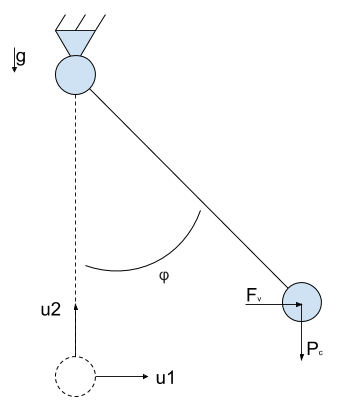
\includegraphics[width=0.27\textwidth]{Pendulo.png}
	\caption{Esquema simplificado del problema}
	\label{pendulo}
\end{figure}


En la figura \ref{pendulo}, $u_1$ corresponde al desplazamiento horizontal de la unión entre el aislador y el cable, $u_2$ al desplazamiento vertical y $P_c=2 \frac{m_cg}{2}$ el peso del cable que debe soportar el aislador. Los perfiles de velocidad en \cite{stengel2017measurements}, correspondientes a ráfagas descendentes alemanas experimentalmente se corroboran como planos. Estos  muestran una pequeña variación a medida que se avanza en la coordenada axial del conductor, como consecuencia $F_v=\frac{1}{2}\rho (T)C_d(Re)d_cu_m^2(z,t)L_c$ donde los valores de $c_d$ y $\rho$ se adjuntan en el código. 

\subsubsection{Perfil de velocidad de viento}
El perfil de velocidad media de viento se obtuvo de \cite{stengel2017measurements} y presenta la siguiente forma:


\begin{figure}[h]
	\centering
	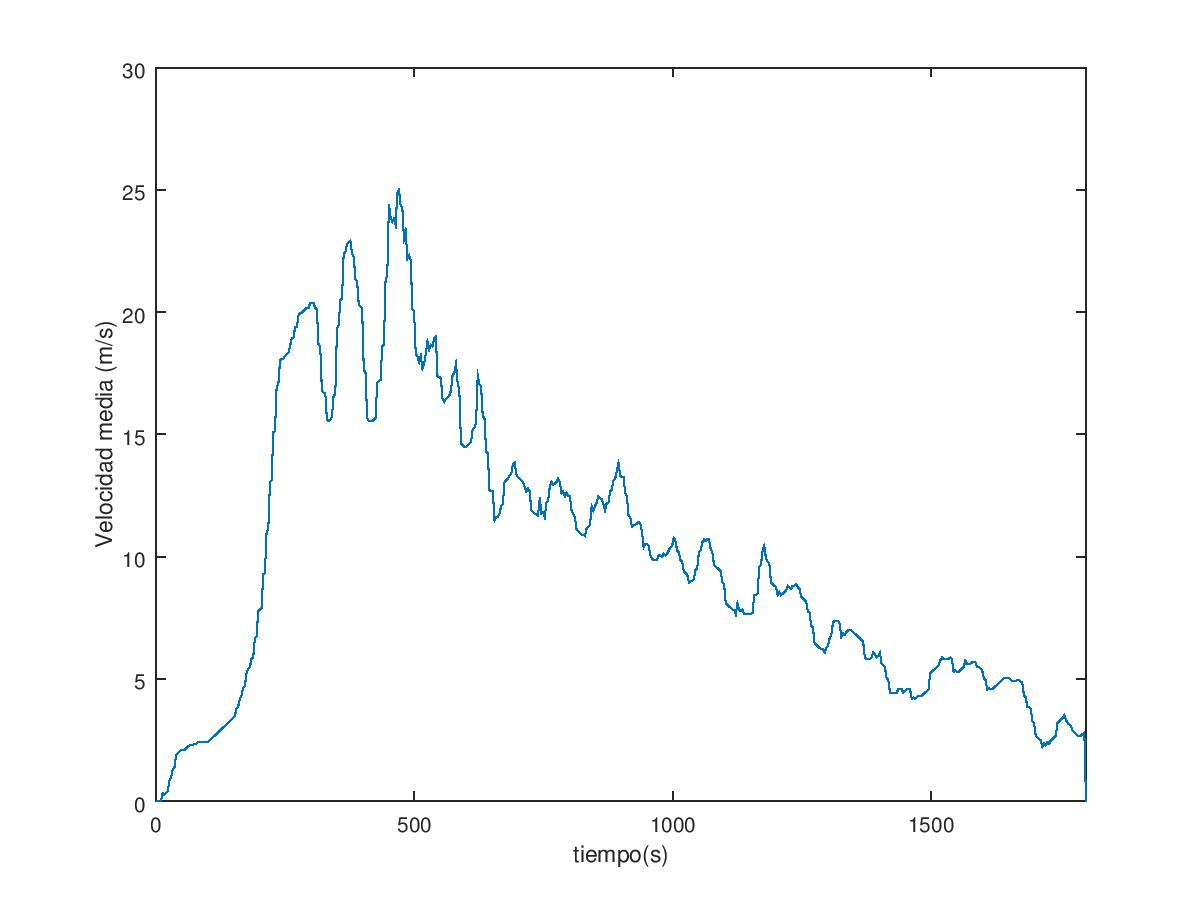
\includegraphics[width=0.6\textwidth]{velocidad.jpg}
	\caption{Perfil de velocidad media a lo largo del cable según \cite{stengel2017measurements}}
\end{figure}

El perfil de velocidades anterior presenta una clara característica de tormenta convectiva descendente, la velocidad aumenta fuertemente en los primeros 500 segundos para luego ir descendiendo de forma gradual. Otra evidencia de este fenómeno es el descenso abrupto de temperatura en cualquiera de las fases, al producirse un régimen de mayor velocidad, aumenta el coeficiente de convención forzada reduciéndose la temperatura de la fase.  En Uruguay estos eventos de interrupción eléctrica de las lineas se debe principalmente a tormentas conectivas. El mismo fenómeno se ha reconocido en Brasil desde hace cierto tiempo, este pone en exigencia estructural a los cables como a las torres \cite{Riera2012}.

\subsubsection{Resultados del modelo}
Las ecuaciones de movimiento para los dos grados de libertad del problema son : 
\begin{eqnarray}
	\frac{m}{2}\ddot{u_1}  +c\dot{u_1}+K_{11}u_1+K_{12}u_2&=&F_v(t)\\
	\frac{m}{2}\ddot{u_2}  +c\dot{u_2}+K_{21}u_1+K_{22}u_2&=&P_c
\end{eqnarray}




El problema reducido anterior presenta condiciones de borde cinemáticas impuestas por la unión entre la torre y la cadena, se agregan el reposo $ {u_{t0}}=0 $, $\dot{u_{t0}}=0$ y la aceleración inicial del movimiento espejo ficticio en $t =-\Delta t $. La resolución se realizó mediante el método presentado en la sección 2.2, se ajustó el valor de c para reproducir de forma aceptable la curva del angulo superpuesta con \cite{stengel2017measurements}, la expresión de este es: 
\begin{equation}
	\varphi =\arctan\left ( \frac{u_1}{u_2} \right ) \cong \arctan\left ( \frac{F_v}{P_c} \right ) 
\end{equation}

La aproximación de que el ángulo va en el sentido de la fuerza externa se basa en el hechos de ser un elemento de biela y que las aceleraciones son nulas, esta hipótesis puede ser considerada en instantes donde el movimiento posee fuerzas no inerciales pequeñas. Para tiempos donde varíe fuertemente la acción externa del viento esta hipótesis no se verifica y se pueden presentar desviaciones en el ángulo. A continuación se muestra  la curva del ángulo medio contrastada con \cite{stengel2017measurements}, donde, mediante ensayo y error se ajusto el valor de $c$ que mejor aproxima dicha curva:


\begin{figure}[h]
	\centering
	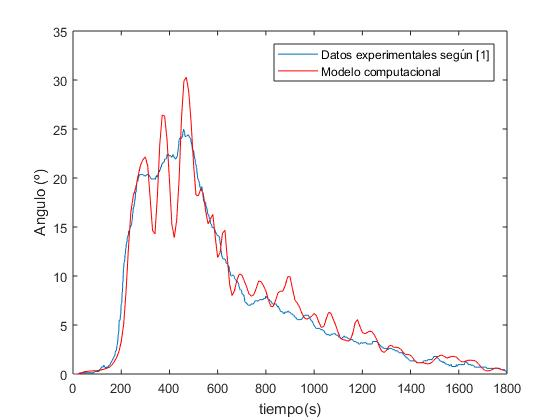
\includegraphics[width=0.6\textwidth]{Angulomedio.jpg}
	\caption{Angulo medio del modelo en contraste con  \cite{stengel2017measurements}   }
\end{figure}

Como se dijo anteriormente el modelo presentado en  \cite{stengel2017measurements} supone hipótesis de un análisis estático, entre los 230 y 500 segundos se producen fuertes variaciones y las mayores velocidades de viento esto puede dar lugar a las desviaciones mostradas en la figura anterior. Estas últimas, en contra partida, reproducen correctamente el ángulo máximo de balanceo, sin aplicar la media móvil, medido en \cite{stengel2017measurements}, valor que permite predecir la aproximación de la cadena a la torre y por tanto cuando se produciría la salida en servicio de la linea. 

Con el objetivo de reducir el ruido en el ángulo y velocidad se escogió una media móvil de acuerdo con \cite{stengel2017measurements}. Este periodo debe ser tal que se produzca una velocidad media relativamente suave, sin perder la forma de la señal ni eliminar completamente la característica de aleatoriedad en la componente fluctuante de la velocidad. Para este caso se eligió una media móvil de 30 segundos.
%agregar referencia 6 que es el 6 del paper aleman

Otro resultado el cual vale analizar es el defasaje que presenta la fuerza del viento con el ángulo debido a la inercia del sistema. Si definimos una función compleja $H(\omega)$ tal que $H(\omega)F=X$ donde $F$ representa el módulo de la fuerza y $X$ el vector complejo de desplazamiento solución a la oscilación forzada, proyectándolo en el eje real se obtiene el valor de $X(t)$. El vector complejo $H(\omega)$ presenta cierto ángulo, esto es consecuencia del defasaje entre la respuesta del sistema y su forzante $F$. En la siguiente figura se evidencia dicho retraso en el tiempo de la respuesta del sistema ($ \varphi) $ en naranja y en azul el valor de $F$ .


\begin{figure}[h]
	\centering
	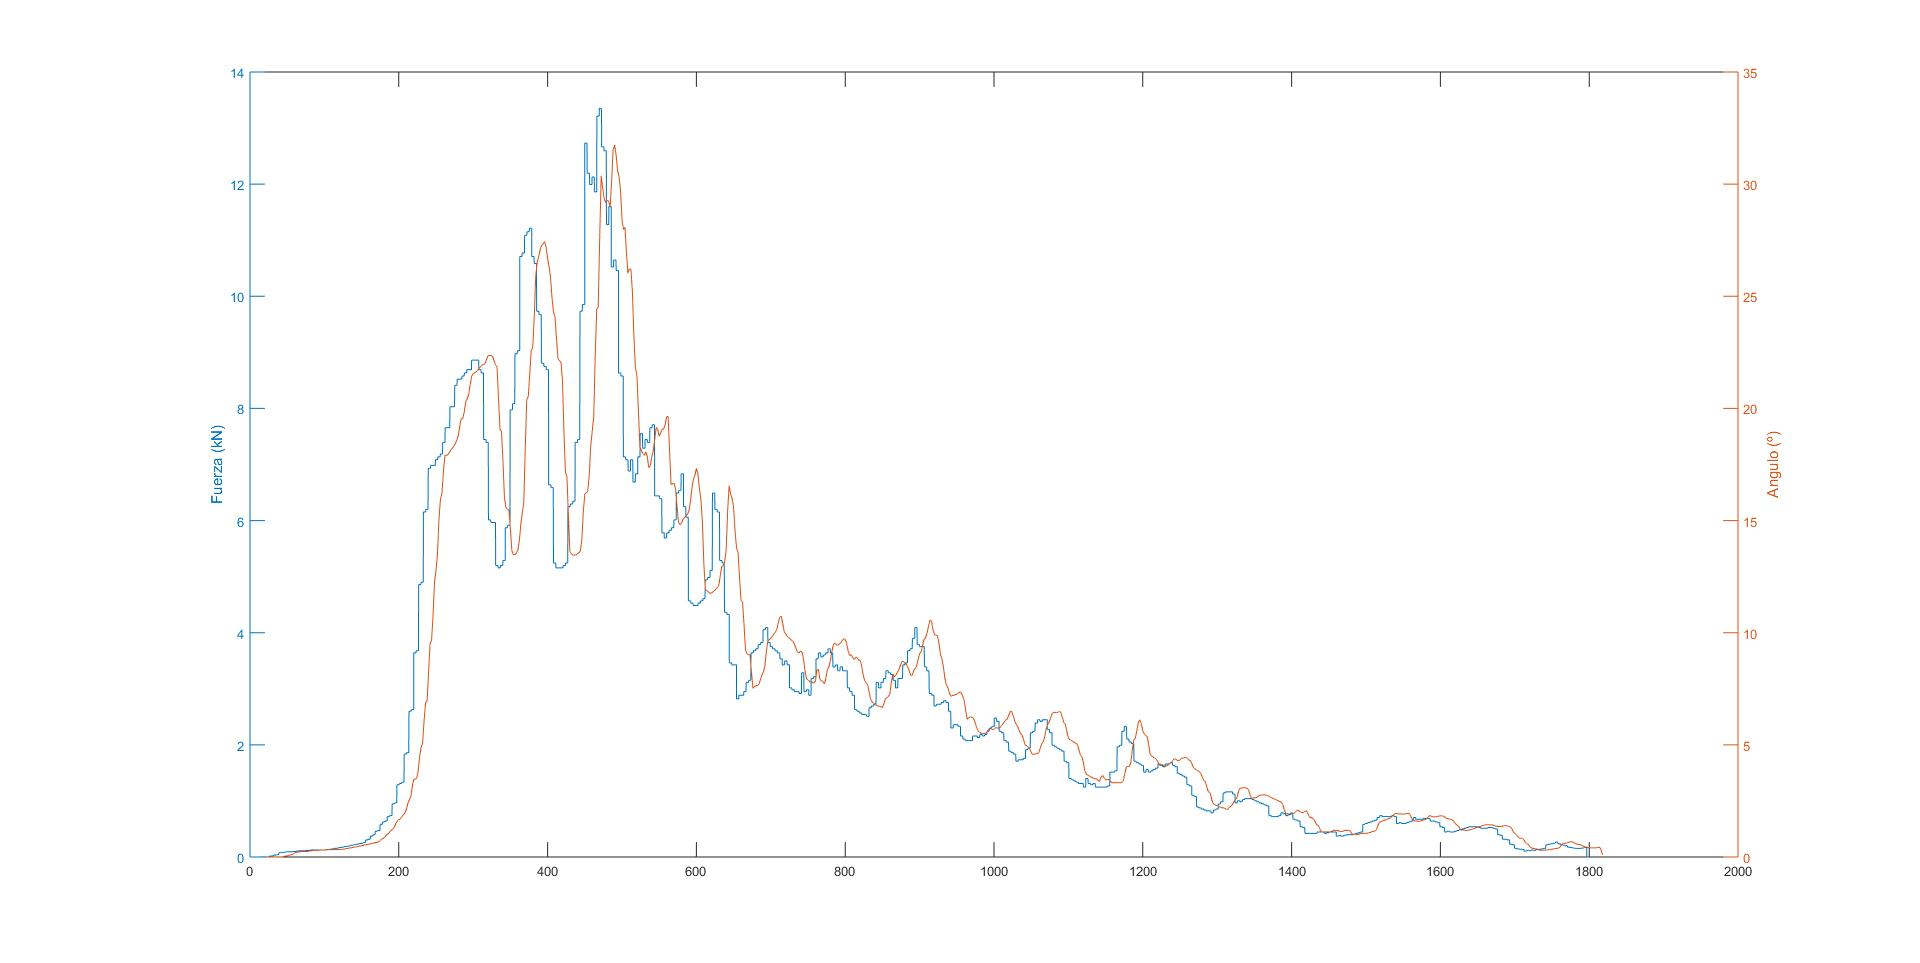
\includegraphics[width=0.8\textwidth]{FuerzaAngulo.jpg}
	\caption{Curva desfajase ángulo fuerza}
\end{figure}


Se realizó un análisis modal como fue presentado en la sección 2.3, las frecuencias naturales asociadas al aislador son de:
\begin{eqnarray}
	f_1&=&0.03Hz\\
	f_2&=&83Hz
\end{eqnarray}


La primer frecuencia presenta un vector propio   $(\varphi_1)=(1,0)$ siendo la primer componente del vector  la asociada con $u_1$ y la segunda entrada  $u_2$. Claramente  $(\varphi_2)=(0,1)$, esto se debe a que los vectores son lineal mente independientes y que es el movimiento restante dinámicamente posible. Se hace notar el hecho de que que las componentes estén desacopladas, es decir que $(\varphi_2).(\varphi_1)=0$, es consecuencia de que los modos se hallaron en un entorno de la posición $\varphi=0$, solo con la acción de la gravedad donde $K_T=K_{T1}$.

\subsection{Resultados numéricos 3D}
Se procede a resolver el problema en tres dimensiones. El sistema se compone de dos cadenas de aisladores y un cable. Las cadenas de aisladores serán modeladas como una biela, el nodo superior de esta permanece fijo mientras que al otro se le asignan dos grados de libertad (desplazamientos en y, z), esto se debe a que hacia ambos lados del cable continuarían cables idénticos haciendo que este punto no tenga desplazamientos en el sentido de x. El cable será representado como un conjunto de barras articuladas en sus extremos como se muestra en la figura \ref{13dddddd}, con tres grados de libertad en sus nodos, exceptuando la unión con el aislador (nodos 2 y n-1).


\begin{figure}[h]
	\centering
	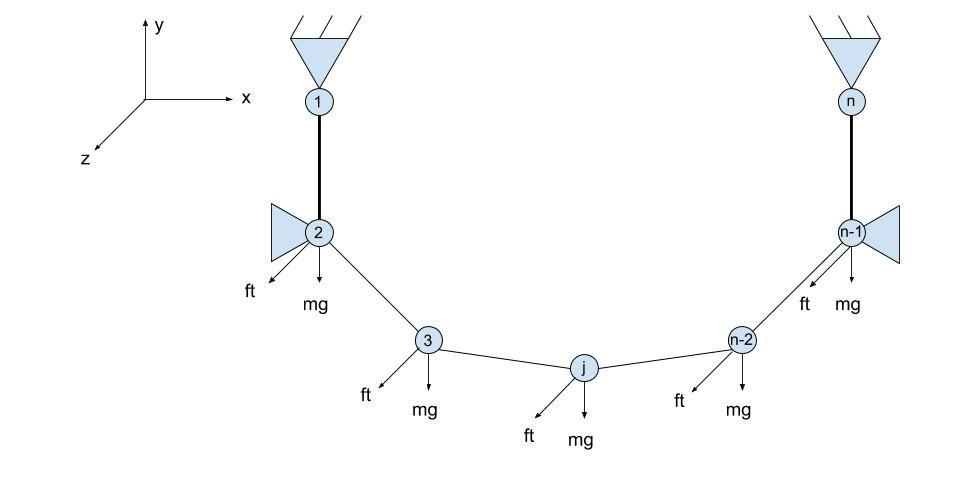
\includegraphics[width=0.8\textwidth]{1.jpg}
	\caption{Esquema simplificado del problema 3D}
	\label{13dddddd}
\end{figure}

Para esta parte se deberá contar con matrices cuadradas de (nx3), siendo n el numero de barras. Esto genera un compromiso a la hora de elegir n, dado que simular el cable con un número pequeño de barras no representa al mismo y un numero extenso de estas hará que la simulación sea de gran costo computacional logrando un modelo más realista, incluso existen casos donde no es posible lograr una simulación. El método de resolución seguirá siendo por diferencias centradas donde la matriz de masa quedará diagonal repartiendo la mitad de la masa en cada uno de sus nodos.


\subsection{Frecuencias naturales}
En una primera instancia son calculados los modos para este sistema. Los mismos son calculados en la posición natural del cable, por lo que se debe realizar una simulación donde la única fuerza que actúa es la gravedad, aplicada sobre los nodos, y se logre alcanzar el equilibrio. La particularidad está dada en que la matriz de rigidez es calculada como la matriz tangente no lineal, por lo que se debe conocer los desplazamientos una vez cargado el cable.
\begin{equation}
	K_T=K_{T1}+K_{T2}+K_{\sigma} 
\end{equation}
Una vez hallada esta matriz se procede a calcular las frecuencias naturales y los modos del sistema a partir de la ecuación ya mencionada $(K-\lambda.M).\phi = 0$. Se puede observar que los modos revelados por este estudio son en diferentes planos y con frecuencias pequeñas asociadas, en comparación con modelos de estructuras.
Se presentan a continuación las primeras 5 frecuencias naturales del sistema e imágenes ilustrando los modos asociados a ellas en el anexo. Además se adjuntan vídeos del movimiento asociados con los mismos.
\begin{itemize}
	\item $1^a - 0.0908 Hz$
	\item $2^a - 0.1815 Hz$
	\item $3^a - 0.1818 Hz$
	\item $4^a - 0.2658 Hz$
	\item $5^a - 0.2721 Hz$
\end{itemize}



El estudio se centra en la primera de las frecuencias, 0.091 Hz, ya que su modo asociado es el que genera mayor desplazamiento horizontal en la cadena de aisladores. A continuación se presenta el primer modo con el mayor de los desplazamientos a 15 metros de la posición original para mejor visualización. En azul se esboza el cable en su posición natural y en rojo el primer modo asociado.

\begin{figure}[h]
	\centering
	\label{2}
	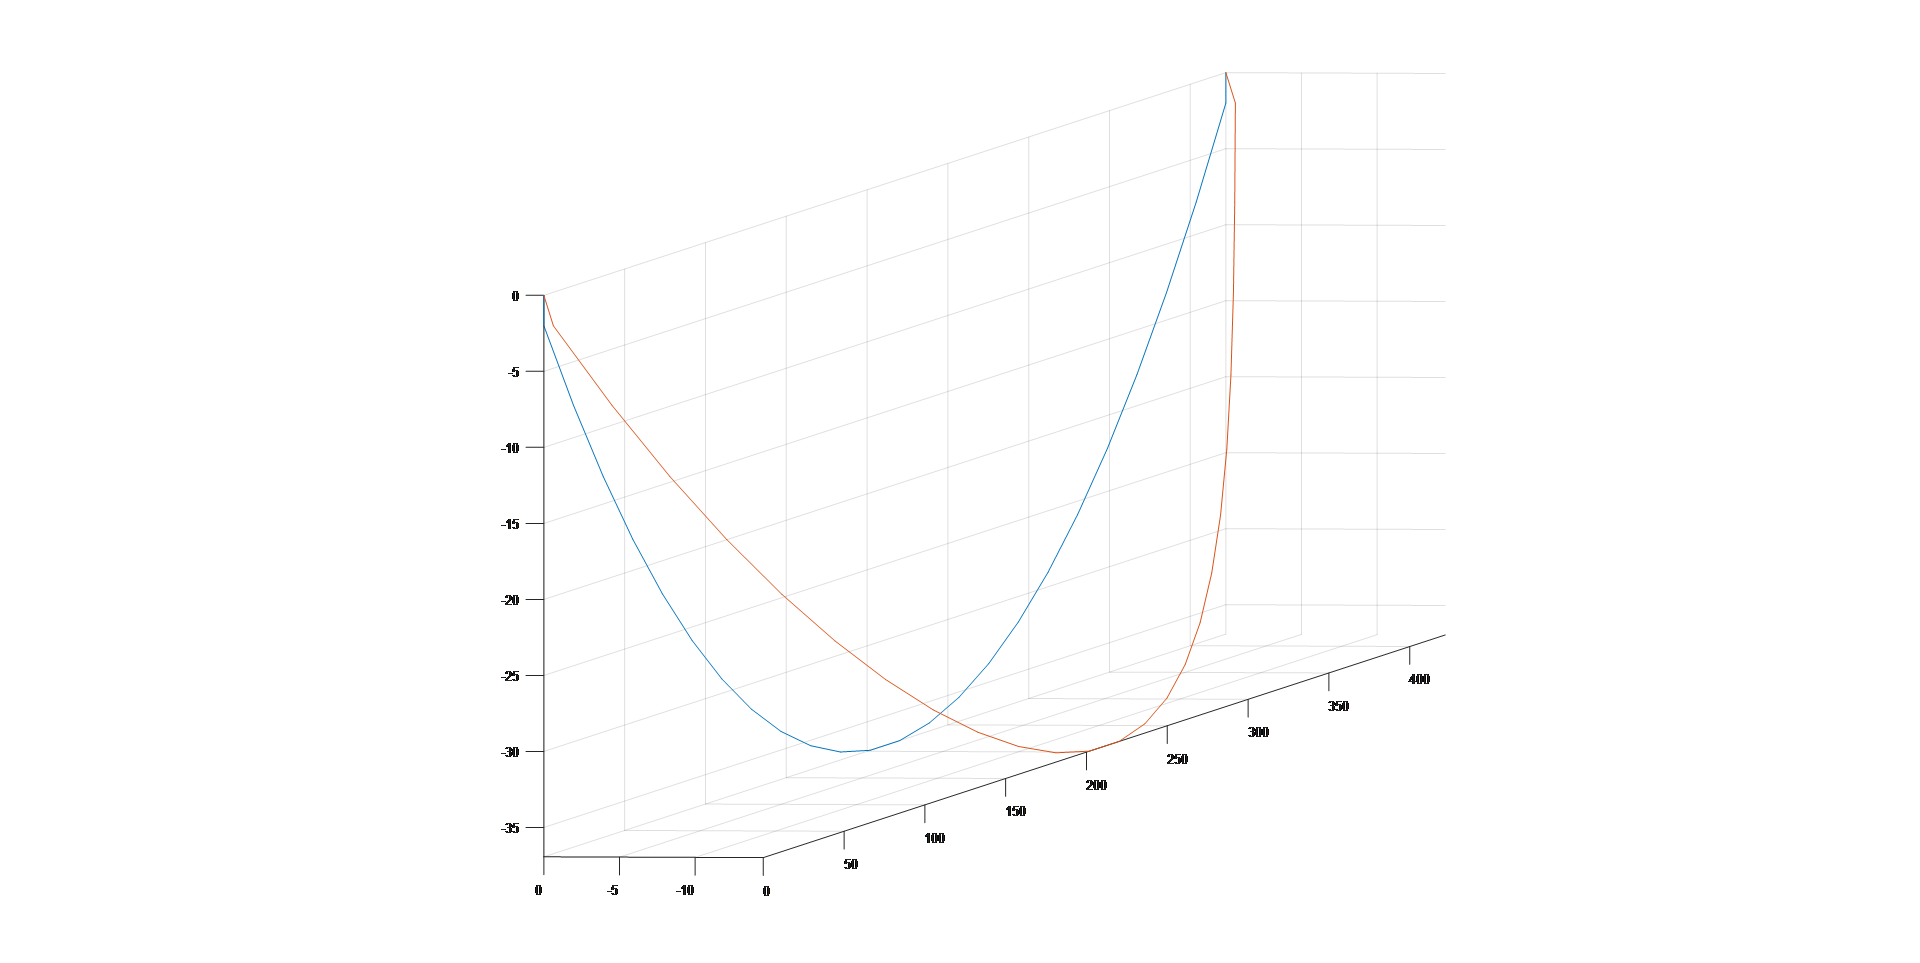
\includegraphics[width=0.85\textwidth]{2.png}
	\caption{Configuración adoptada por el primer modo.}
\end{figure}




El planteo consta en excitar el cable con una fuerza sinusoidal con frecuencia igual a la menor de las frecuencias naturales, pretendiendo disminuir los desplazamientos de la cadena de aisladores colocando masas concentradas de 80 kg en determinados puntos del cable. Es por esto que se simula el cable en 4 instancias diferentes aumentando la masa de determinados nodos. Los nodos seleccionados para colocar las masas son:
\begin{itemize}
	\item Los dos que se encuentran vinculados a la cadena de aisladores.
	\item Los dos ubicados a $\frac{1}{6}$ de la distancia horizontal de entre aisladores.
	\item Los dos ubicados a $\frac{2}{6}$ de la distancia horizontal de entre aisladores.
	\item En el nodo central con dos masas.
\end{itemize}





\begin{figure}[h]
	\centering
	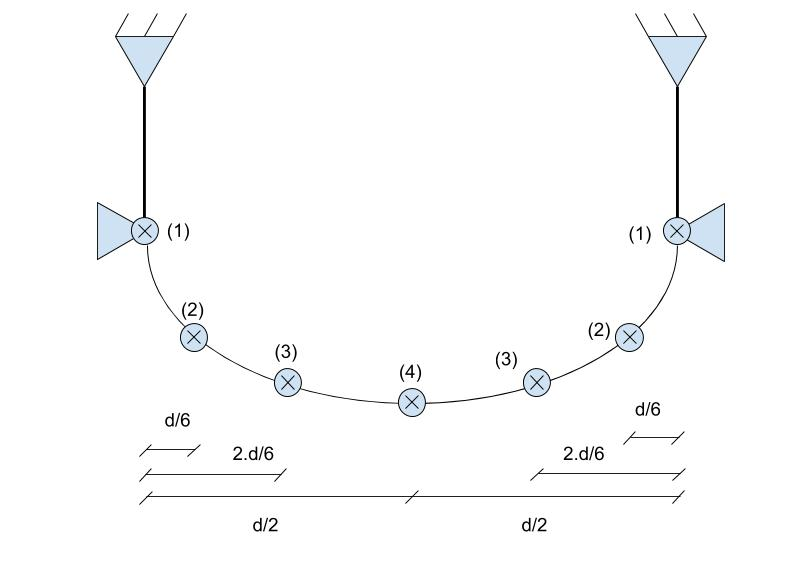
\includegraphics[width=0.5\textwidth]{cable_masas.jpg}
	\caption{Distribución de masas colocadas.}
	\label{masas}
\end{figure}




\newpage
Mediante estas cuatro simulaciones se constató que la mejor solución para este problema es colocar las dos masas concentradas en el medio del cable. Con esto se logra una reducción en el desplazamiento horizontal de la cadena de aisladores de aproximadamente un 85\% para un transitorio de 1500 segundos. A continuación se presenta el desplazamiento del nodo estudiado antes y después de colocar las masas.


La respuestas en el tiempo para la fuerza sinusoidal de frecuencia igual al primer modo se presenta en las figuras: \ref{desphorizsinm}, \ref{angulosinm}.

\begin{figure}[h]
	\centering
	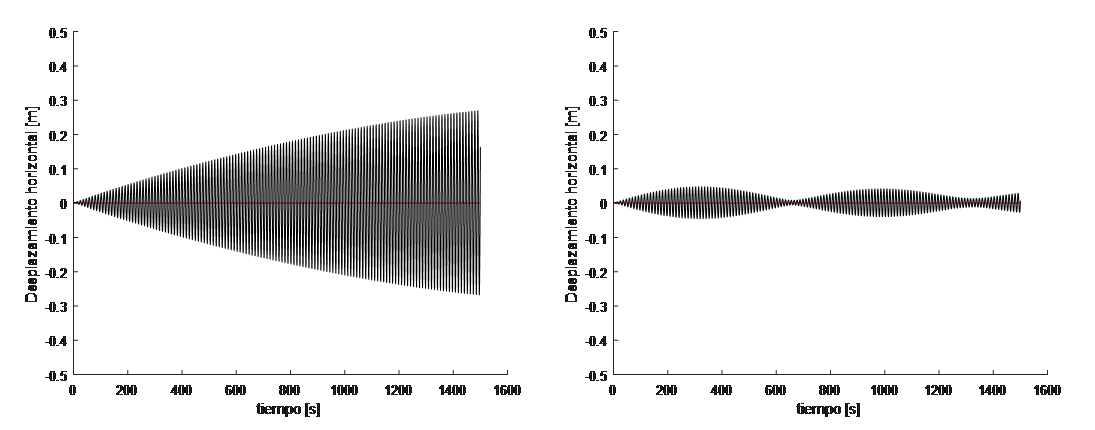
\includegraphics[width=0.8\textwidth]{34.png}
	\caption{Desplazamiento horizontal de la cadena de aisladora en función del tiempo con y sin masas.}
	\label{desphorizsinm}
\end{figure}

\begin{figure}[h]
	\centering
	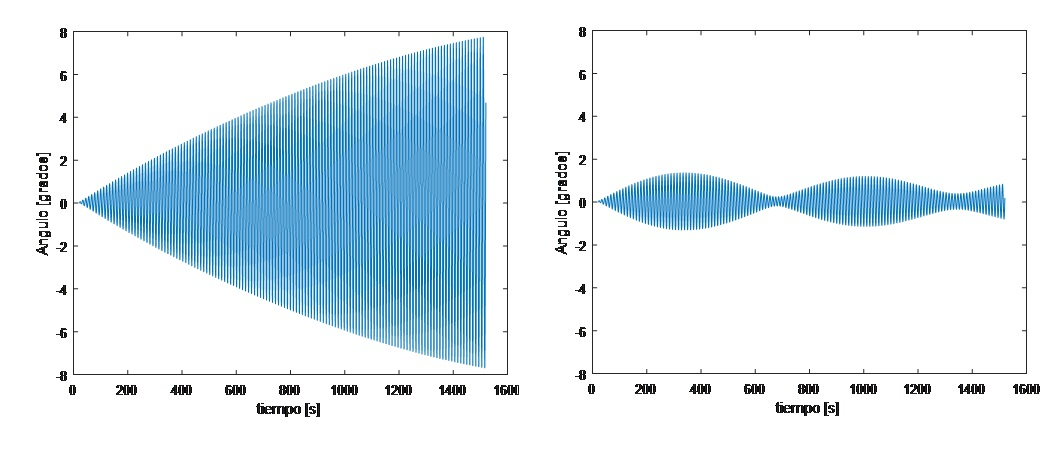
\includegraphics[width=0.8\textwidth]{56.jpg}
	\caption{Ángulo de la cadena de aisladora en función del tiempo con y sin masas.}
	\label{angulosinm}
\end{figure}






Por un lado, la opción de colocar masas en el cable puede parecer muy fácil de implementar y ayudaría a que los desplazamientos del cable disminuyan de forma considerable para fuerzas de este tipo en particular, pero no hay que dejar de evaluar otros cambios que se pueden generar a partir de este método. Se debe considerar que tanto las torres como la cadena de aisladores quedaran sometidas a un peso mayor, en este caso se trata de un aumento de 160 Kg, en cada uno de los cables, donde se deberá tener en cuenta las normas aplicadas por UTE si es factible este tipo de soluciones.
Por otra parte, se debe considerar que cambian las frecuencias naturales del nuevo sistema. Se presentan las cinco primeras frecuencias naturales sin masas agregadas y con masas aplicadas en el nodo central:

\begin{itemize}
	\item $1^a - 0.0908 Hz \rightarrow 1^a - 0.0893 Hz$
	\item $2^a - 0.1815 Hz \rightarrow 2^a - 0.1908 Hz$
	\item $3^a - 0.1818 Hz \rightarrow 3^a - 0.1913 Hz$
	\item $4^a - 0.2658 Hz \rightarrow 4^a - 0.2622 Hz$
	\item $5^a - 0.2721 Hz \rightarrow 5^a - 0.2685 Hz$
\end{itemize}



Se observa que la primera frecuencia natural disminuye un 2\%, esto hace que la frecuencia con la que se aplica la fuerza en el estudio anterior es próxima a la frecuencia natural del nuevo sistema, de igual manera los desplazamientos se atenúan de forma considerable.

\subsection{Respuesta a tormenta convectiva}

En esta instancia se somete al cable a fuerzas ejercidas por el viento. Al igual que en el caso del péndulo, las velocidades y fuerzas ejercidas por el viento son obtenidas a partir de \cite{stengel2017measurements}. Dadas estas condiciones, se compara el movimiento del nodo móvil de la cadena de aisladores contra lo documentado en el artículo antes mencionado, y los resultados arrojados de la simulación Péndulo. Para esto se consideraron los mismos parámetros que en el modelo 2D.A continuación se presenta el ángulo respecto de la vertical que forma la cadena de aisladores en función del tiempo al aplicarle la fuerza ejercida por el viento:



\begin{figure}[h]
	\centering
	\label{anguotiempo3d}
	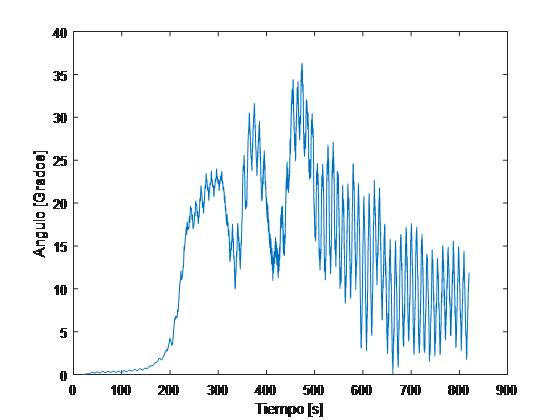
\includegraphics[width=0.5\textwidth]{7.png}
	\caption{Respuesta del angulo de la cadena de aisladora en función del tiempo.}
\end{figure}


En la siguiente figura se comparan los resultados arrojados del angulo con los datos de \cite{stengel2017measurements}. Para luego a través de una media móvil filtrar los datos obtenidos.


\begin{figure}[h]
	\centering
	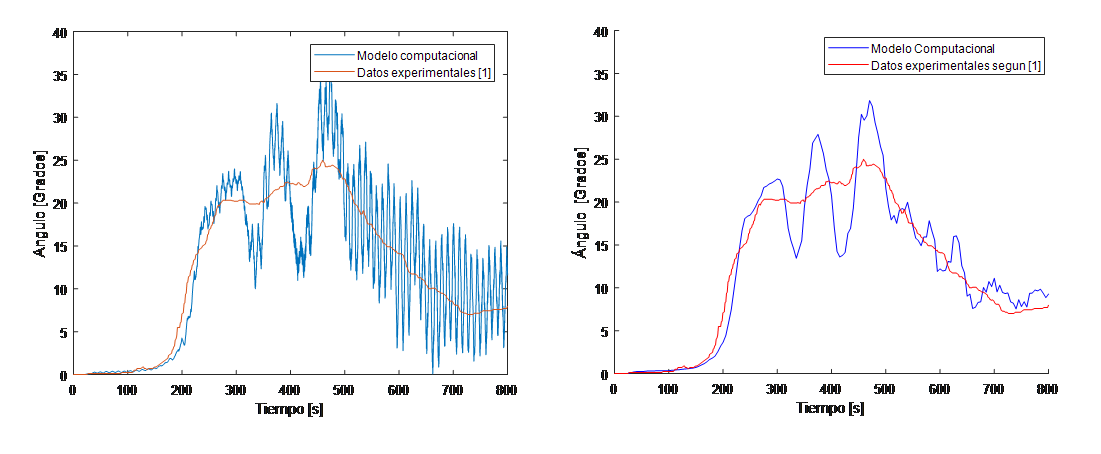
\includegraphics[width=0.85\textwidth]{89.png}
	\caption{Datos del ángulo sin procesar y luego de aplicarle una media móvil}
	\label{21}
\end{figure}


Cuando se compara con los datos arrojados por \cite{stengel2017measurements}, se pude apreciar la misma distorsión que ocurría en la simulación 2D. Esta cambio significativo se puede deber a no tener precisamente los mismos datos que se utilizaron en \cite{stengel2017measurements}. De todas formas el programa tiene la misma tendencia a comportarse como los datos de referencia al aplicarle el viento. 

\newpage
Comparando los resultados con el modelo 2D se puede observar que las curvas descritas por ambos modelos reflejan el mismo comportamiento:

\begin{figure}[h]
	\centering
	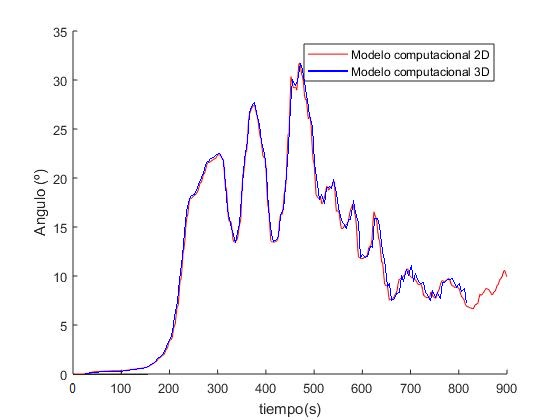
\includegraphics[width=0.5\textwidth]{superpesta.jpg}
	\caption{Contraste de los modelos 2D/3D}
	\label{2dvs3d}
\end{figure}

Los datos arrojados por el modelo Péndulo y 3D difieren en menos de un 5\% para cada posición en el tiempo. La gran diferencia que existen entre estas dos simulaciones es que en el para el caso 2D se debe asumir que las fuerzas son homogéneas en todo el cable y se puede ver que representa bien esta situación.  Las tormentas conectivas son homogéneas en toda la extensión del cable por lo que el programa puede servir para simulaciones futuras.



Por último, se procede a aplicarle al sistema una masa de 160 Kg en el medio del cable, como en la primera simulación 3D, excitándolo con la fuerza del viento para conocer los desplazamientos del nodo móvil de la cadena de aisladores.(Figura \ref{respuestaconmasas}).


\begin{figure}[h]
	\centering
	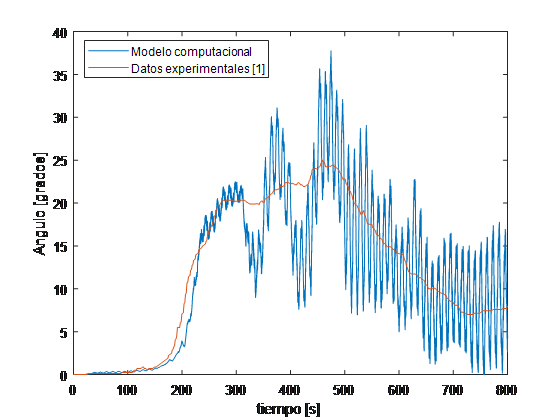
\includegraphics[width=0.5\textwidth]{10.png}
	\caption{Respuesta del ángulo para tormenta convectiva utilizando una media móvil y masas sobre el cable}
	\label{respuestaconmasas}
\end{figure}

A partir de los datos anteriores se puede ver que no existen grandes cambios en el movimiento del nodo libre en la cadena de aisladores cuando se aplica una fuerza proveniente de una tormenta conectiva al añadirle una masa de 160 kg en el centro del cable. Para este tipo de problemas no sería de gran ayuda la solución que se había encontrado en el la primera parte de esta sección.